
% Article - значит без глав, только секции
\documentclass{article}
\usepackage{lmodern}
% Задаем шрифты
\usepackage{fontspec}
\setmainfont[Scale=1.4]{Times New Roman} % Главный шрифт
\setmonofont[Scale=1.0]{Consolas} % Моноширинный шрифт

% Поддержка русского языка (переносов, орфографии)
\usepackage{polyglossia}
\usepackage{microtype} % better management of overfulls
\usepackage{ucharclasses}

\setmainlanguage{russian} % Ставим русский главным
\setotherlanguage{english} % Английский второстепенным
% Отступы по ГОСТу
\usepackage{geometry}
\geometry{
	a4paper,
	left=3cm,
	top=2cm,
	bottom=2cm,
	right=1cm,
}

\usepackage{setspace}
\hyphenpenalty=1000 % default 50
\tolerance=500      % default 200

\setTransitionsForLatin{\begingroup\hyphenrules{english}}{\endgroup}

% Можно вставлять скрипты на Lua (компилить через lualatex)
%\usepackage{luacode}

% Example
% \begin{luacode}
% tex.print(math.random())
% \end{luacode}
\begin{hyphenrules}{russian}
\hyphenation{веб-фрейм-ворк}
\end{hyphenrules}

\usepackage{listings}
\lstset{
  basicstyle=\ttfamily,
  keywordstyle=\ttfamily,
  stringstyle=\ttfamily,
  commentstyle=\ttfamily,
  breaklines=true,
  keepspaces=true,
  extendedchars=\true
}


\usepackage{python}


%%% ТИТУЛЬНИК %%%
%%%%%%%%%%%%%%%%%
\newcommand{\entityintro}[3]{%
  \hbox to \hsize{%
    \vbox{%
      \hbox to .2in{}%
    }%
    {\bf  #1}%
    \dotfill\pageref{#2}%
  }
  \makebox[\hsize]{%
    \parbox{.4in}{}%
    \parbox[l]{5in}{%
      \vspace{1mm}%
      #3%
      \vspace{1mm}%
    }%
  }%
}


\newcommand{\refdefined}[1]{
\expandafter\ifx\csname r@#1\endcsname\relax
\relax\else
{$($стр. \pageref{#1}$)$}\fi}



\begin{document}
% Отключаем нумерацию страниц
\pagenumbering{gobble}
\begin{center}

МИНИСТЕРСТВО ОБРАЗОВАНИЯ И НАУКИ РОССИЙСКОЙ ФЕДЕРАЦИИ
НОВОСИБИРСКИЙ ГОСУДАРСТВЕННЫЙ ТЕХНИЧЕСКИЙ УНИВЕРСИТЕТ
ФАКУЛЬТЕТ АВТОМАТИКИ И ВЫЧИСЛИТЕЛЬНОЙ ТЕХНИКИ
КАФЕДРА ВЫЧИСЛИТЕЛЬНОЙ ТЕХНИКИ

\vspace{\fill}
{\bfseries \Large Расчетно-графическая работа}

{\itshape по дисциплине <<Современные информационные технологии>>}

на тему <<Одностраничное Web-приложение>>

\vspace{\fill}

\begin{flushleft}
\begin{tabular}{ l l }
Студент & Кузьмин Д.С. \\
Группа & АВТ-318 \\
Преподаватель & Васюткина И.А. \\
\end{tabular}
\end{flushleft}

\vspace{\fill}
Новосибирск 2015 г.
\end{center}
\pagebreak

% Включаем нумерацию страниц
\pagenumbering{arabic}

%%% СЕКЦИИ %%%
%%%%%%%%%%%%%%
\tableofcontents
\pagebreak
\section{Цель работы}
\doublespacing

Разработать одностраничное веб-приложение с использованием веб-фрейворка Vaadin для отображения 
информации о погоде в различных городах, курсе валют и кол-ве посещений страницы приложения


\section{Техническое задание}
\doublespacing

\begin{enumerate}

\item При создании приложения использоть веб-фрейворк Vaadin для создания интерфейса и взаимодействия между клиентом и сервером.
\item Реализовать получение и парсинг данных прогноза погоды на текущий и завтрашний день с сервиса ForecastIO
\item Реализовать получение и парсинг данных о курсах валют (доллар США, евро) с сайта ЦентроБанка России
\item Реализовать учет числа посещений страницы во время работы приложения (уникальные посетители, общее число посещений)
\item Добавить возможность обновлять данные из пунктов выше вручную по нажатию кнопки без перезагрузки страницы
\item Показывать IP-адрес пользователя, находящегося на странице
\item Показывать на странице время последнего обновления данных
\item Хранить информацию о посещениях из NoSQL БД Mongo

\end{enumerate}

\section{Проектирование}
\doublespacing

Была спрроектирована следующая структура классов:

\begin{figure}[h]
\centering
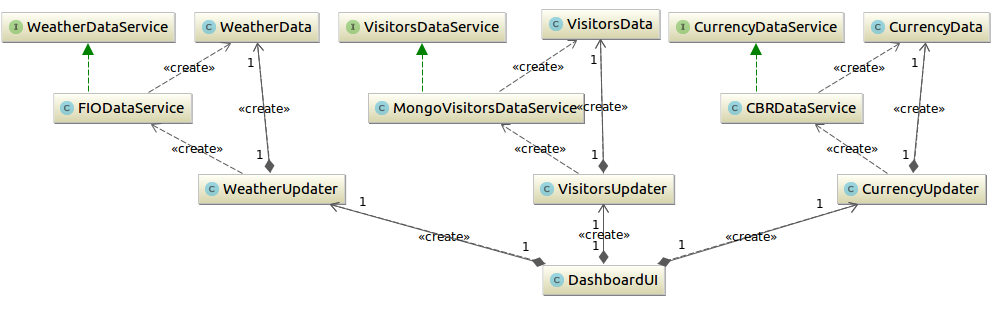
\includegraphics[width=\textwidth]{uml}
\caption{Диаграмма классов проекта}
\end{figure}

Краткое описание реализованных абстракций:
\begin{itemize}
\item Классы типа <<DataService>> работают непосредственно с источниками данных (база данных, сторонние сервисы). Результатом их работы является класс с полезной информацией типа <<Data>>
\item Классы типа <<Data>> содержат в себе информацию, необходимую и достаточную для ее отображения в графическом интерфейсе без дополнительных запросов к посторонним модулям.
\item Классы типа <<Updater>> реализуют функционал обновления графических компонентов, предобрабатывая и передавая информацию из классов типа <<Data>> этим компонентам.
\item Класс DashboardUI является корневым классом проекта. Он напрямую взаимодействует с фреймворком Vaadin - инициализирует интерфейс и является насленидком его класса шаблона. Этот класс имеет внутренний класс DashboardUIServlet, который является 
наследником HttpServlet и привязывается к контейнеру сервлетов аннотацией фреймворка.
\end{itemize}

Привозникновении непредвиженных ситуаций, пользователю сообщается 
об ошибке в сплывающей панели.

\section{Описание пользовательского интерфейса}
\doublespacing

\begin{figure}[h]
\centering
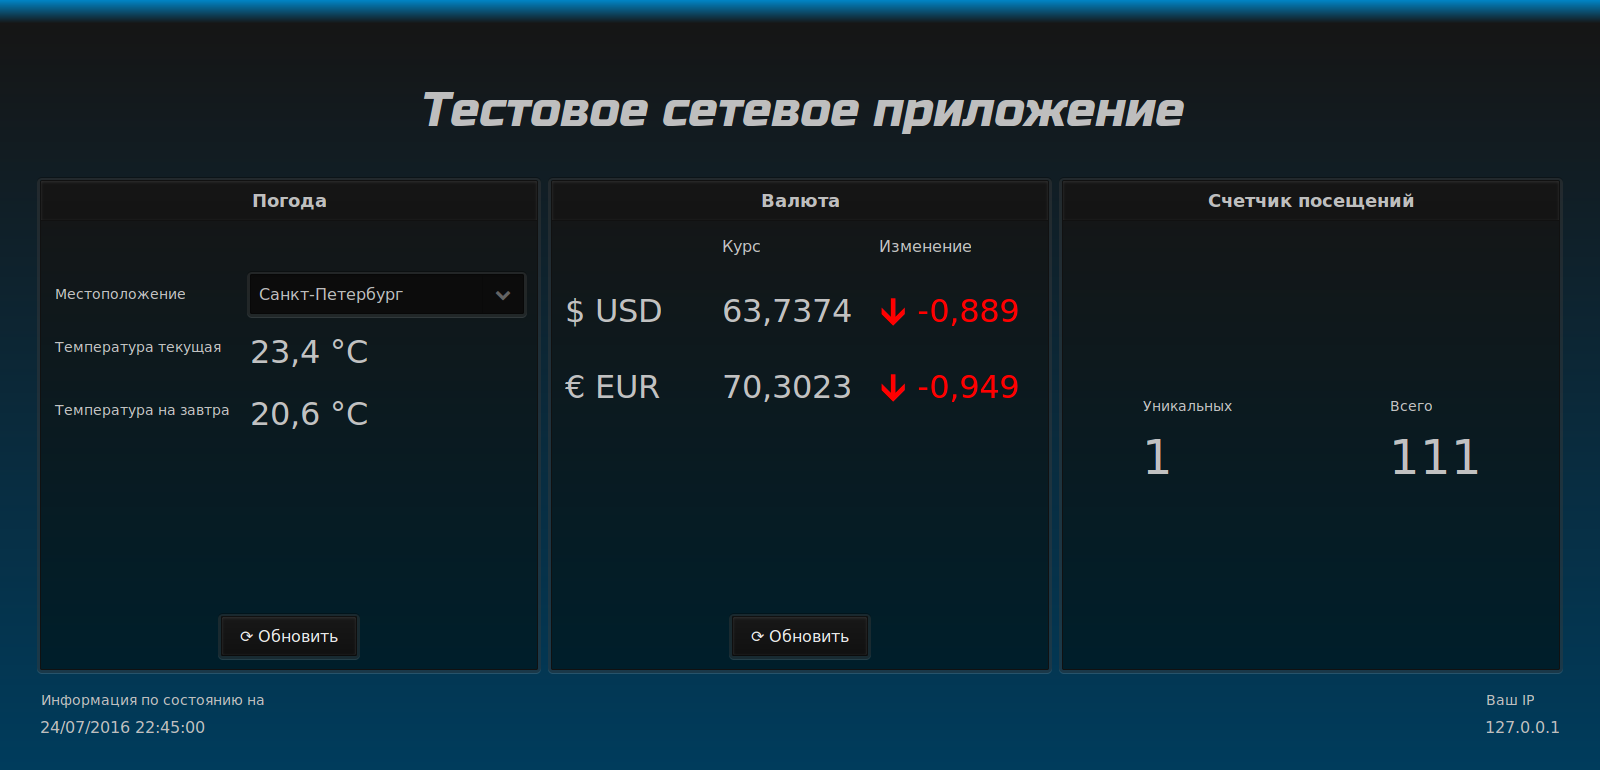
\includegraphics[width=\textwidth]{screenshot}
\caption{Скриншот приложения}
\label{fig:screen1}
\end{figure}

Представление информации на стороне клиента показано на рисунке \ref{fig:screen1}.
На странице расположены 3 панели


\begin{itemize}
\item На левой панели отображается информация о погоде. В выпадающем списке можно выбрать населенный пункт,
по которому будет загружаться информация. Доступно 3 населенных пункта - Москва, Санкт-Петербург и Новосибирск.
Чуть ниже выводится температура в градусах по Цельсию на сегодняшний и завтрашний календарные дни. При смене пункта в выпадающем списке для применения изменений необходимо кликнуть по кнопке <<Обновить>>.
\item На средней панели отображается информация о текущей валюте - эквивалент Американского доллара и Евро в Российских рублях под колонкой <<Курс>> и изменение этого значения с момента последнего обновления в Центральном Банке России (обычно 1-3 дней) под  колонкой <<Изменение>>. Для обновления значений необходимо кликнуть по кнопке <<Обновить>> внизу панели.
\item На правой панели отображается счеткик посещений данной страницы. Под колонкой <<Уникальных>> отображено число уникальных посетителей, загрузивших данную страницу. Под колонкой <<Всего>> отображается общее количество посещений этой страницы.
\end{itemize}

В правом нижнем углу отображается текущий IP-адрес пользователя, загрузившего текущую страницу.

В левом нижнем углу отображается время последнего обновления любой из 2х панелей - о погоде либо о курсе валют. Либо с момента последеней перезагрузки страницы.

\section{Структурное описание разработки}

\subsection*{Пакет com.xotonic.dashboard.weather}{
\label{com.xotonic.dashboard.weather}\hskip -.05in
\hbox to \hsize{\textit{ Структура\hfil Стр.}}
\vskip .13in
\hbox{{\bf  Интерфейсы}}
\entityintro{WeatherDataService}{com.xotonic.dashboard.weather.WeatherDataService}{Интерфейс для взаимодействия с \texttt{\small DashboardUI}{\small 
\refdefined{com.xotonic.dashboard.ui.DashboardUI}}}
\vskip .13in
\hbox{{\bf  Классы}}
\entityintro{Cities}{com.xotonic.dashboard.weather.Cities}{Список городов}
\entityintro{FIODataService}{com.xotonic.dashboard.weather.FIODataService}{Загрузчик прогноза погоды с forecast.io.}
\entityintro{WeatherData}{com.xotonic.dashboard.weather.WeatherData}{Класс для передачи информации от загрузчиков погодных информеров (\texttt{\small WeatherDataService}{\small 
\refdefined{com.xotonic.dashboard.weather.WeatherDataService}})}
\vskip .1in
\vskip .1in
\subsubsection*{\label{com.xotonic.dashboard.weather.WeatherDataService}Интерфейс WeatherDataService}{
\vskip .1in 
Интерфейс для взаимодействия с \texttt{\small DashboardUI}{\small 
\refdefined{com.xotonic.dashboard.ui.DashboardUI}}\vskip .1in 
\subsubsection*{Объявление}{
\begin{lstlisting}[frame=none]
public interface WeatherDataService
\end{lstlisting}

\subsubsection*{Реализуют}{FIODataService\small{\refdefined{com.xotonic.dashboard.weather.FIODataService}}}
\subsubsection*{Методы}{
\vskip -2em
\begin{itemize}
\item{ 
\index{getData(Cities)}
{\bf  getData}\\
\begin{lstlisting}[frame=none]
WeatherData getData(Cities city) throws com.xotonic.dashboard.ExceptionForUser\end{lstlisting} %end signature
\begin{itemize}
\item{
{\bf  Параметры}
  \begin{itemize}
   \item{
\texttt{city} -- Запрашиваемый город}
  \end{itemize}
}%end item
\item{{\bf  Возвращемое значение} -- 
Информация по этому городу 
}%end item
\item{{\bf  Выбрасывает исключение}
  \begin{itemize}
   \item{\vskip -.6ex \texttt{com.xotonic.dashboard.ExceptionForUser} -- }
  \end{itemize}
}%end item
\end{itemize}
}%end item
\end{itemize}
}
}
\subsubsection*{\label{com.xotonic.dashboard.weather.Cities}Класс Cities}{
\vskip .1in 
Список городов\vskip .1in 
\subsubsection*{Объявление}{
\begin{lstlisting}[frame=none]
public final Класс Cities
 extends java.lang.Enum\end{lstlisting}
\subsubsection*{Поля}{
\begin{itemize}
\item{
\index{MSK}
\label{com.xotonic.dashboard.weather.Cities.MSK}\texttt{public static final Cities\ {\bf  MSK}}
\begin{itemize}
\item{\vskip -.9ex 
Москва}
\end{itemize}
}
\item{
\index{SPB}
\label{com.xotonic.dashboard.weather.Cities.SPB}\texttt{public static final Cities\ {\bf  SPB}}
\begin{itemize}
\item{\vskip -.9ex 
Санкт-Петебург}
\end{itemize}
}
\item{
\index{NSK}
\label{com.xotonic.dashboard.weather.Cities.NSK}\texttt{public static final Cities\ {\bf  NSK}}
\begin{itemize}
\item{\vskip -.9ex 
Новосибирск}
\end{itemize}
}
\end{itemize}
}
\subsubsection*{Конструкторы}{
\vskip -2em
\begin{itemize}
\item{ 
\index{Cities()}
{\bf  Cities}\\
\begin{lstlisting}[frame=none]
private Cities()\end{lstlisting} %end signature
}%end item
\end{itemize}
}
\subsubsection*{Методы}{
\vskip -2em
\begin{itemize}
\item{ 
\index{byID(int)}
{\bf  byID}\\
\begin{lstlisting}[frame=none]
public static Cities byID(int id)\end{lstlisting} %end signature
\begin{itemize}
\item{
{\bf  Описание}

Вернуть город по порядковому номеру в списке
}
\item{
{\bf  Параметры}
  \begin{itemize}
   \item{
\texttt{id} -- номер в списке}
  \end{itemize}
}%end item
\item{{\bf  Возвращемое значение} -- 
 
}%end item
\end{itemize}
}%end item
\item{ 
\index{valueOf(String)}
{\bf  valueOf}\\
\begin{lstlisting}[frame=none]
public static Cities valueOf(java.lang.String name)\end{lstlisting} %end signature
}%end item
\item{ 
\index{values()}
{\bf  values}\\
\begin{lstlisting}[frame=none]
public static Cities[] values()\end{lstlisting} %end signature
}%end item
\end{itemize}
}
}
\subsubsection*{\label{com.xotonic.dashboard.weather.FIODataService}Класс FIODataService}{
\vskip .1in 
Загрузчик прогноза погоды с forecast.io.\mbox{}\newline Следует помнить, что сервис предоставляет ограниченноое количество запросов (всего 1000 единовременно)\vskip .1in 
\subsubsection*{Объявление}{
\begin{lstlisting}[frame=none]
public class FIODataService
 extends java.lang.Object implements WeatherDataService\end{lstlisting}
\subsubsection*{Поля}{
\begin{itemize}
\item{
\index{APPKEY}
\label{com.xotonic.dashboard.weather.FIODataService.APPKEY}\texttt{private static final java.lang.String\ {\bf  APPKEY}}
\begin{itemize}
\item{\vskip -.9ex 
Бесплатный APIKEY (ключ разработчика)}
\end{itemize}
}
\item{
\index{lats}
\label{com.xotonic.dashboard.weather.FIODataService.lats}\texttt{private static final java.lang.String\lbrack \rbrack \ {\bf  lats}}
\begin{itemize}
\item{\vskip -.9ex 
Широты городов}
\end{itemize}
}
\item{
\index{lons}
\label{com.xotonic.dashboard.weather.FIODataService.lons}\texttt{private static final java.lang.String\lbrack \rbrack \ {\bf  lons}}
\begin{itemize}
\item{\vskip -.9ex 
Долготы городов}
\end{itemize}
}
\end{itemize}
}
\subsubsection*{Конструкторы}{
\vskip -2em
\begin{itemize}
\item{ 
\index{FIODataService()}
{\bf  FIODataService}\\
\begin{lstlisting}[frame=none]
public FIODataService()\end{lstlisting} %end signature
}%end item
\end{itemize}
}
\subsubsection*{Методы}{
\vskip -2em
\begin{itemize}
\item{ 
\index{getData(Cities)}
{\bf  getData}\\
\begin{lstlisting}[frame=none]
public WeatherData getData(Cities city) throws com.xotonic.dashboard.ExceptionForUser\end{lstlisting} %end signature
\begin{itemize}
\item{
{\bf  Описание}

Получить информацию о погоде в конкретном городе
}
\item{
{\bf  Параметры}
  \begin{itemize}
   \item{
\texttt{city} -- Запрашиваемый город}
  \end{itemize}
}%end item
\item{{\bf  Возвращемое значение} -- 
 
}%end item
\item{{\bf  Выбрасывает исключение}
  \begin{itemize}
   \item{\vskip -.6ex \texttt{com.xotonic.dashboard.ExceptionForUser} -- }
  \end{itemize}
}%end item
\end{itemize}
}%end item
\end{itemize}
}
}
\subsubsection*{\label{com.xotonic.dashboard.weather.WeatherData}Класс WeatherData}{
\vskip .1in 
Класс для передачи информации от загрузчиков погодных информеров (\texttt{\small WeatherDataService}{\small 
\refdefined{com.xotonic.dashboard.weather.WeatherDataService}})\vskip .1in 
\subsubsection*{Объявление}{
\begin{lstlisting}[frame=none]
public class WeatherData
 extends java.lang.Object\end{lstlisting}
\subsubsection*{Поля}{
\begin{itemize}
\item{
\index{celcium\_today}
\label{com.xotonic.dashboard.weather.WeatherData.celcium_today}\texttt{public float\ {\bf  celcium\_today}}
\begin{itemize}
\item{\vskip -.9ex 
Значение температуры за сегодня в градусах по Цельсию}
\end{itemize}
}
\item{
\index{celcium\_tomorrow}
\label{com.xotonic.dashboard.weather.WeatherData.celcium_tomorrow}\texttt{public float\ {\bf  celcium\_tomorrow}}
\begin{itemize}
\item{\vskip -.9ex 
Значение температуры на завтра в градусах по Цельсию}
\end{itemize}
}
\item{
\index{city}
\label{com.xotonic.dashboard.weather.WeatherData.city}\texttt{public Cities\ {\bf  city}}
\begin{itemize}
\item{\vskip -.9ex 
Город, для которого предназначен прогноз}
\end{itemize}
}
\end{itemize}
}
\subsubsection*{Конструкторы}{
\vskip -2em
\begin{itemize}
\item{ 
\index{WeatherData()}
{\bf  WeatherData}\\
\begin{lstlisting}[frame=none]
public WeatherData()\end{lstlisting} %end signature
}%end item
\end{itemize}
}
}
}
\subsection*{Пакет com.xotonic.dashboard.currency}{
\label{com.xotonic.dashboard.currency}\hskip -.05in
\hbox to \hsize{\textit{ Структура\hfil Стр.}}
\vskip .13in
\hbox{{\bf  Интерфейсы}}
\entityintro{CurrencyDataService}{com.xotonic.dashboard.currency.CurrencyDataService}{Интерфейс для службы получения курса валют}
\vskip .13in
\hbox{{\bf  Классы}}
\entityintro{CBRDataService}{com.xotonic.dashboard.currency.CBRDataService}{Парсинг курса валют с сайта Центрального Банка России}
\entityintro{CurrencyData}{com.xotonic.dashboard.currency.CurrencyData}{Класс, содержащий информацию о курсе валют}
\vskip .1in
\vskip .1in
\subsubsection*{\label{com.xotonic.dashboard.currency.CurrencyDataService}Интерфейс CurrencyDataService}{
\vskip .1in 
Интерфейс для службы получения курса валют\vskip .1in 
\subsubsection*{Объявление}{
\begin{lstlisting}[frame=none]
public interface CurrencyDataService
\end{lstlisting}

\subsubsection*{Реализуют}{CBRDataService\small{\refdefined{com.xotonic.dashboard.currency.CBRDataService}}}
\subsubsection*{Методы}{
\vskip -2em
\begin{itemize}
\item{ 
\index{getData()}
{\bf  getData}\\
\begin{lstlisting}[frame=none]
CurrencyData getData() throws com.xotonic.dashboard.ExceptionForUser\end{lstlisting} %end signature
}%end item
\end{itemize}
}
}
\subsubsection*{\label{com.xotonic.dashboard.currency.CBRDataService}Класс CBRDataService}{
\vskip .1in 
Парсинг курса валют с сайта Центрального Банка России\vskip .1in 
\subsubsection*{Объявление}{
\begin{lstlisting}[frame=none]
public class CBRDataService
 extends java.lang.Object implements CurrencyDataService\end{lstlisting}
\subsubsection*{Поля}{
\begin{itemize}
\item{
\index{ID\_USD}
\label{com.xotonic.dashboard.currency.CBRDataService.ID_USD}\texttt{private final java.lang.String\ {\bf  ID\_USD}}
\begin{itemize}
\item{\vskip -.9ex 
Уникальный код Американского доллара в XML}
\end{itemize}
}
\item{
\index{ID\_EUR}
\label{com.xotonic.dashboard.currency.CBRDataService.ID_EUR}\texttt{private final java.lang.String\ {\bf  ID\_EUR}}
\begin{itemize}
\item{\vskip -.9ex 
Уникальный код Евро в XML}
\end{itemize}
}
\item{
\index{URL}
\label{com.xotonic.dashboard.currency.CBRDataService.URL}\texttt{private final java.lang.String\ {\bf  URL}}
\begin{itemize}
\item{\vskip -.9ex 
URL запроса к Центробанку}
\end{itemize}
}
\end{itemize}
}
\subsubsection*{Конструкторы}{
\vskip -2em
\begin{itemize}
\item{ 
\index{CBRDataService()}
{\bf  CBRDataService}\\
\begin{lstlisting}[frame=none]
public CBRDataService()\end{lstlisting} %end signature
}%end item
\end{itemize}
}
\subsubsection*{Методы}{
\vskip -2em
\begin{itemize}
\item{ 
\index{buildUrl(Date, Date, String)}
{\bf  buildUrl}\\
\begin{lstlisting}[frame=none]
private java.lang.String buildUrl(java.util.Date from,java.util.Date to,java.lang.String id)\end{lstlisting} %end signature
\begin{itemize}
\item{
{\bf  Описание}

Вставить в URL параметры запроса
}
\item{
{\bf  Параметры}
  \begin{itemize}
   \item{
\texttt{from} -- Начальная дата}
   \item{
\texttt{to} -- Конечная дата}
   \item{
\texttt{id} -- Идентификатор валюты}
  \end{itemize}
}%end item
\item{{\bf  Возвращемое значение} -- 
Готовый URL для отправки на сервер ЦБ 
}%end item
\end{itemize}
}%end item
\item{ 
\index{getData()}
{\bf  getData}\\
\begin{lstlisting}[frame=none]
public CurrencyData getData() throws com.xotonic.dashboard.ExceptionForUser\end{lstlisting} %end signature
\begin{itemize}
\item{
{\bf  Описание}

Выполнить запрос на сайт Центробанка по обеим валютам
}
\item{{\bf  Возвращемое значение} -- 
Информация о валюте 
}%end item
\item{{\bf  Выбрасывает исключение}
  \begin{itemize}
   \item{\vskip -.6ex \texttt{com.xotonic.dashboard.ExceptionForUser} -- }
  \end{itemize}
}%end item
\end{itemize}
}%end item
\item{ 
\index{setLastWorkingDay(Calendar)}
{\bf  setLastWorkingDay}\\
\begin{lstlisting}[frame=none]
private void setLastWorkingDay(java.util.Calendar cal)\end{lstlisting} %end signature
\begin{itemize}
\item{
{\bf  Описание}

Найти последний рабочий день в ЦБ
}
\item{
{\bf  Параметры}
  \begin{itemize}
   \item{
\texttt{cal} -- }
  \end{itemize}
}%end item
\end{itemize}
}%end item
\end{itemize}
}
}
\subsubsection*{\label{com.xotonic.dashboard.currency.CurrencyData}Класс CurrencyData}{
\vskip .1in 
Класс, содержащий информацию о курсе валют\vskip .1in 
\subsubsection*{Объявление}{
\begin{lstlisting}[frame=none]
public class CurrencyData
 extends java.lang.Object\end{lstlisting}
\subsubsection*{Поля}{
\begin{itemize}
\item{
\index{EUR}
\label{com.xotonic.dashboard.currency.CurrencyData.EUR}\texttt{public float\ {\bf  EUR}}
\begin{itemize}
\item{\vskip -.9ex 
Курс евро по отношению к рублю}
\end{itemize}
}
\item{
\index{EURDelta}
\label{com.xotonic.dashboard.currency.CurrencyData.EURDelta}\texttt{public float\ {\bf  EURDelta}}
\begin{itemize}
\item{\vskip -.9ex 
Изменение евро}
\end{itemize}
}
\item{
\index{USD}
\label{com.xotonic.dashboard.currency.CurrencyData.USD}\texttt{public float\ {\bf  USD}}
\begin{itemize}
\item{\vskip -.9ex 
Курс доллара по отношению к рублю}
\end{itemize}
}
\item{
\index{USDDelta}
\label{com.xotonic.dashboard.currency.CurrencyData.USDDelta}\texttt{public float\ {\bf  USDDelta}}
\begin{itemize}
\item{\vskip -.9ex 
Изменение доллара}
\end{itemize}
}
\end{itemize}
}
\subsubsection*{Конструкторы}{
\vskip -2em
\begin{itemize}
\item{ 
\index{CurrencyData()}
{\bf  CurrencyData}\\
\begin{lstlisting}[frame=none]
public CurrencyData()\end{lstlisting} %end signature
}%end item
\end{itemize}
}
}
}
\subsection*{Пакет com.xotonic.dashboard.ui}{
\label{com.xotonic.dashboard.ui}\hskip -.05in
\hbox to \hsize{\textit{ Структура\hfil Стр.}}
\vskip .13in
\hbox{{\bf  Классы}}
\entityintro{CurrencyUpdater}{com.xotonic.dashboard.ui.CurrencyUpdater}{Обновление курса валют\mbox{}\newline }
\entityintro{DashboardUI}{com.xotonic.dashboard.ui.DashboardUI}{Отрисовка UI и управление событиями}
\entityintro{DashboardUI.DashboardUIServlet}{com.xotonic.dashboard.ui.DashboardUI.DashboardUIServlet}{Сервлет приложения}
\entityintro{VisitorsUpdater}{com.xotonic.dashboard.ui.VisitorsUpdater}{Обновление счетчика посещения\mbox{}\newline }
\entityintro{WeatherUpdater}{com.xotonic.dashboard.ui.WeatherUpdater}{Обновление прогноза погоды\mbox{}\newline }
\vskip .1in
\vskip .1in
\subsubsection*{\label{com.xotonic.dashboard.ui.CurrencyUpdater}Класс CurrencyUpdater}{
\vskip .1in 
Обновление курса валют\mbox{}\newline \vskip .1in 
\subsubsection*{Объявление}{
\begin{lstlisting}[frame=none]
public class CurrencyUpdater
 extends java.lang.Object implements com.vaadin.ui.Button.ClickListener, java.lang.Runnable\end{lstlisting}
\subsubsection*{Поля}{
\begin{itemize}
\item{
\index{usdLabel}
\label{com.xotonic.dashboard.ui.CurrencyUpdater.usdLabel}\texttt{private final com.vaadin.ui.Label\ {\bf  usdLabel}}
\begin{itemize}
\item{\vskip -.9ex 
Надпись для значения текущего курса доллара}
\end{itemize}
}
\item{
\index{usdDeltaLabel}
\label{com.xotonic.dashboard.ui.CurrencyUpdater.usdDeltaLabel}\texttt{private final com.vaadin.ui.Label\ {\bf  usdDeltaLabel}}
\begin{itemize}
\item{\vskip -.9ex 
Надпись для значения изменения текущего курса доллара}
\end{itemize}
}
\item{
\index{eurLabel}
\label{com.xotonic.dashboard.ui.CurrencyUpdater.eurLabel}\texttt{private final com.vaadin.ui.Label\ {\bf  eurLabel}}
\begin{itemize}
\item{\vskip -.9ex 
Надпись для значения текущего курса евро}
\end{itemize}
}
\item{
\index{eurDeltaLabel}
\label{com.xotonic.dashboard.ui.CurrencyUpdater.eurDeltaLabel}\texttt{private final com.vaadin.ui.Label\ {\bf  eurDeltaLabel}}
\begin{itemize}
\item{\vskip -.9ex 
Надпись для значения изменения текущего курса евро}
\end{itemize}
}
\item{
\index{silent}
\label{com.xotonic.dashboard.ui.CurrencyUpdater.silent}\texttt{private boolean\ {\bf  silent}}
\begin{itemize}
\item{\vskip -.9ex 
Метка, отключающая вывод сообщения пользователю об успешном обновлении}
\end{itemize}
}
\item{
\index{timeStatusValueLabel}
\label{com.xotonic.dashboard.ui.CurrencyUpdater.timeStatusValueLabel}\texttt{private final com.vaadin.ui.Label\ {\bf  timeStatusValueLabel}}
\begin{itemize}
\item{\vskip -.9ex 
Надпись с временем последнего обновления}
\end{itemize}
}
\item{
\index{currencyFormat}
\label{com.xotonic.dashboard.ui.CurrencyUpdater.currencyFormat}\texttt{private final java.text.DecimalFormat\ {\bf  currencyFormat}}
\begin{itemize}
\item{\vskip -.9ex 
Форматирование для строк с числовыми значениями курса}
\end{itemize}
}
\item{
\index{currencyDeltaFormat}
\label{com.xotonic.dashboard.ui.CurrencyUpdater.currencyDeltaFormat}\texttt{private final java.text.DecimalFormat\ {\bf  currencyDeltaFormat}}
\begin{itemize}
\item{\vskip -.9ex 
Форматирование для строк с числовыми значениями изменения курса}
\end{itemize}
}
\item{
\index{currencyData}
\label{com.xotonic.dashboard.ui.CurrencyUpdater.currencyData}\texttt{private com.xotonic.dashboard.currency.CurrencyData\ {\bf  currencyData}}
\begin{itemize}
\item{\vskip -.9ex 
Информация о текущем курсе}
\end{itemize}
}
\end{itemize}
}
\subsubsection*{Конструкторы}{
\vskip -2em
\begin{itemize}
\item{ 
\index{CurrencyUpdater(Label, Label, Label, Label, Label)}
{\bf  CurrencyUpdater}\\
\begin{lstlisting}[frame=none]
public CurrencyUpdater(com.vaadin.ui.Label usdLabel,com.vaadin.ui.Label usdDeltaLabel,com.vaadin.ui.Label eurLabel,com.vaadin.ui.Label eurDeltaLabel,com.vaadin.ui.Label timeStatusValueLabel)\end{lstlisting} %end signature
\begin{itemize}
\item{
{\bf  Описание}

Конструктор
}
\item{
{\bf  Параметры}
  \begin{itemize}
   \item{
\texttt{usdLabel} -- курс доллара}
   \item{
\texttt{usdDeltaLabel} -- изменение курса доллара}
   \item{
\texttt{eurLabel} -- курс евро}
   \item{
\texttt{eurDeltaLabel} -- изменение курса евро}
   \item{
\texttt{timeStatusValueLabel} -- дата и время, которое обновится после получения новых данных}
  \end{itemize}
}%end item
\end{itemize}
}%end item
\end{itemize}
}
\subsubsection*{Методы}{
\vskip -2em
\begin{itemize}
\item{ 
\index{buttonClick(Button.ClickEvent)}
{\bf  buttonClick}\\
\begin{lstlisting}[frame=none]
public void buttonClick(com.vaadin.ui.Button.ClickEvent event)\end{lstlisting} %end signature
\begin{itemize}
\item{
{\bf  Описание}

Обработчик клика по кнопке 'Обновить'
}
\item{
{\bf  Параметры}
  \begin{itemize}
   \item{
\texttt{event} -- }
  \end{itemize}
}%end item
\end{itemize}
}%end item
\item{ 
\index{isSilent()}
{\bf  isSilent}\\
\begin{lstlisting}[frame=none]
public boolean isSilent()\end{lstlisting} %end signature
\begin{itemize}
\item{
{\bf  Описание}

Вернуть флаг, включающий оповещение пользователя об успешном обновлении
}
\end{itemize}
}%end item
\item{ 
\index{run()}
{\bf  run}\\
\begin{lstlisting}[frame=none]
public void run()\end{lstlisting} %end signature
\begin{itemize}
\item{
{\bf  Описание}

Эмуляция нажатия на кнопку обновления при запуске класса как Runnable
}
\end{itemize}
}%end item
\item{ 
\index{setSilent(boolean)}
{\bf  setSilent}\\
\begin{lstlisting}[frame=none]
public void setSilent(boolean silent)\end{lstlisting} %end signature
\begin{itemize}
\item{
{\bf  Описание}

Поставить флаг, включающий оповещение пользователя об успешном обновлении
}
\end{itemize}
}%end item
\item{ 
\index{updateCurrency()}
{\bf  updateCurrency}\\
\begin{lstlisting}[frame=none]
private void updateCurrency()\end{lstlisting} %end signature
\begin{itemize}
\item{
{\bf  Описание}

Обновить информацию о курсе валют
}
\end{itemize}
}%end item
\item{ 
\index{updateDateLabel()}
{\bf  updateDateLabel}\\
\begin{lstlisting}[frame=none]
private void updateDateLabel()\end{lstlisting} %end signature
\begin{itemize}
\item{
{\bf  Описание}

Обновить текст с временем последнего обновления
}
\end{itemize}
}%end item
\end{itemize}
}
}
\subsubsection*{\label{com.xotonic.dashboard.ui.DashboardUI}Класс DashboardUI}{
\vskip .1in 
Отрисовка UI и управление событиями\vskip .1in 
\subsubsection*{Объявление}{
\begin{lstlisting}[frame=none]
public class DashboardUI
 extends com.vaadin.ui.UI\end{lstlisting}
\subsubsection*{Поля}{
\begin{itemize}
\item{
\index{weatherUpdater}
\label{com.xotonic.dashboard.ui.DashboardUI.weatherUpdater}\texttt{ WeatherUpdater\ {\bf  weatherUpdater}}
\begin{itemize}
\item{\vskip -.9ex 
Компонент для обновления погоды}
\end{itemize}
}
\item{
\index{currencyUpdater}
\label{com.xotonic.dashboard.ui.DashboardUI.currencyUpdater}\texttt{ CurrencyUpdater\ {\bf  currencyUpdater}}
\begin{itemize}
\item{\vskip -.9ex 
Компонент для обновления курса валют}
\end{itemize}
}
\item{
\index{visitorsUpdater}
\label{com.xotonic.dashboard.ui.DashboardUI.visitorsUpdater}\texttt{ VisitorsUpdater\ {\bf  visitorsUpdater}}
\begin{itemize}
\item{\vskip -.9ex 
Компонент для обновления количества посещений}
\end{itemize}
}
\end{itemize}
}
\subsubsection*{Конструкторы}{
\vskip -2em
\begin{itemize}
\item{ 
\index{DashboardUI()}
{\bf  DashboardUI}\\
\begin{lstlisting}[frame=none]
public DashboardUI()\end{lstlisting} %end signature
}%end item
\end{itemize}
}
\subsubsection*{Методы}{
\vskip -2em
\begin{itemize}
\item{ 
\index{init(VaadinRequest)}
{\bf  init}\\
\begin{lstlisting}[frame=none]
protected void init(com.vaadin.server.VaadinRequest vaadinRequest)\end{lstlisting} %end signature
\begin{itemize}
\item{
{\bf  Описание}

Инициализация приложения
}
\item{
{\bf  Параметры}
  \begin{itemize}
   \item{
\texttt{vaadinRequest} -- обьект класса-обертки HttpRequest}
  \end{itemize}
}%end item
\end{itemize}
}%end item
\end{itemize}
}
}
\subsubsection*{\label{com.xotonic.dashboard.ui.DashboardUI.DashboardUIServlet}Класс DashboardUI.DashboardUIServlet}{
\vskip .1in 
Сервлет приложения\vskip .1in 
\subsubsection*{Объявление}{
\begin{lstlisting}[frame=none]
public static Класс DashboardUI.DashboardUIServlet
 extends com.vaadin.server.VaadinServlet\end{lstlisting}
\subsubsection*{Конструкторы}{
\vskip -2em
\begin{itemize}
\item{ 
\index{DashboardUIServlet()}
{\bf  DashboardUIServlet}\\
\begin{lstlisting}[frame=none]
public DashboardUIServlet()\end{lstlisting} %end signature
}%end item
\end{itemize}
}
}
\subsubsection*{\label{com.xotonic.dashboard.ui.VisitorsUpdater}Класс VisitorsUpdater}{
\vskip .1in 
Обновление счетчика посещения\mbox{}\newline \vskip .1in 
\subsubsection*{Объявление}{
\begin{lstlisting}[frame=none]
public class VisitorsUpdater
 extends java.lang.Object implements com.vaadin.ui.Button.ClickListener, java.lang.Runnable\end{lstlisting}
\subsubsection*{Поля}{
\begin{itemize}
\item{
\index{uniqueLabel}
\label{com.xotonic.dashboard.ui.VisitorsUpdater.uniqueLabel}\texttt{private final com.vaadin.ui.Label\ {\bf  uniqueLabel}}
\begin{itemize}
\item{\vskip -.9ex 
Метка для записи числа уникальных IP}
\end{itemize}
}
\item{
\index{totalLabel}
\label{com.xotonic.dashboard.ui.VisitorsUpdater.totalLabel}\texttt{private final com.vaadin.ui.Label\ {\bf  totalLabel}}
\begin{itemize}
\item{\vskip -.9ex 
Метка для записи общего числа посещений}
\end{itemize}
}
\item{
\index{visitorsData}
\label{com.xotonic.dashboard.ui.VisitorsUpdater.visitorsData}\texttt{private com.xotonic.dashboard.visitors.VisitorsData\ {\bf  visitorsData}}
\begin{itemize}
\item{\vskip -.9ex 
Информация о посещениях}
\end{itemize}
}
\end{itemize}
}
\subsubsection*{Конструкторы}{
\vskip -2em
\begin{itemize}
\item{ 
\index{VisitorsUpdater(Label, Label)}
{\bf  VisitorsUpdater}\\
\begin{lstlisting}[frame=none]
public VisitorsUpdater(com.vaadin.ui.Label uniqueLabel,com.vaadin.ui.Label totalLabel)\end{lstlisting} %end signature
\begin{itemize}
\item{
{\bf  Описание}

Конструктор класса
}
\end{itemize}
}%end item
\end{itemize}
}
\subsubsection*{Методы}{
\vskip -2em
\begin{itemize}
\item{ 
\index{buttonClick(Button.ClickEvent)}
{\bf  buttonClick}\\
\begin{lstlisting}[frame=none]
public void buttonClick(com.vaadin.ui.Button.ClickEvent event)\end{lstlisting} %end signature
\begin{itemize}
\item{
{\bf  Описание}

Обработчик нажатия на кнопку обновить. На данный момент копка отсутсвует, но обработчик используется при перезагрузке страницы
}
\end{itemize}
}%end item
\item{ 
\index{run()}
{\bf  run}\\
\begin{lstlisting}[frame=none]
public void run()\end{lstlisting} %end signature
\begin{itemize}
\item{
{\bf  Описание}

Обновление информации при запуске класса как Runnable
}
\end{itemize}
}%end item
\item{ 
\index{updateVisitors()}
{\bf  updateVisitors}\\
\begin{lstlisting}[frame=none]
private void updateVisitors()\end{lstlisting} %end signature
\begin{itemize}
\item{
{\bf  Описание}

Загрузить данные из базы данных
}
\end{itemize}
}%end item
\item{ 
\index{upsertAddress(String)}
{\bf  upsertAddress}\\
\begin{lstlisting}[frame=none]
private void upsertAddress(java.lang.String ip)\end{lstlisting} %end signature
\begin{itemize}
\item{
{\bf  Описание}

Сохранить IP-адрес в базе данных
}
\item{
{\bf  Параметры}
  \begin{itemize}
   \item{
\texttt{ip} -- IP-адрес}
  \end{itemize}
}%end item
\end{itemize}
}%end item
\end{itemize}
}
}
\subsubsection*{\label{com.xotonic.dashboard.ui.WeatherUpdater}Класс WeatherUpdater}{
\vskip .1in 
Обновление прогноза погоды\mbox{}\newline \vskip .1in 
\subsubsection*{Объявление}{
\begin{lstlisting}[frame=none]
public class WeatherUpdater
 extends java.lang.Object implements com.vaadin.ui.Button.ClickListener, java.lang.Runnable\end{lstlisting}
\subsubsection*{Поля}{
\begin{itemize}
\item{
\index{weatherData}
\label{com.xotonic.dashboard.ui.WeatherUpdater.weatherData}\texttt{private com.xotonic.dashboard.weather.WeatherData\ {\bf  weatherData}}
\begin{itemize}
\item{\vskip -.9ex 
Информация о погоде в определенном населенном пункте}
\end{itemize}
}
\item{
\index{defaultCityId}
\label{com.xotonic.dashboard.ui.WeatherUpdater.defaultCityId}\texttt{public final int\ {\bf  defaultCityId}}
\begin{itemize}
\item{\vskip -.9ex 
НП, который будет загружаться по умолчанию}
\end{itemize}
}
\item{
\index{placeSelect}
\label{com.xotonic.dashboard.ui.WeatherUpdater.placeSelect}\texttt{private final com.vaadin.ui.ComboBox\ {\bf  placeSelect}}
\begin{itemize}
\item{\vskip -.9ex 
Выпадающий список с НП}
\end{itemize}
}
\item{
\index{places}
\label{com.xotonic.dashboard.ui.WeatherUpdater.places}\texttt{private final java.util.ArrayList\ {\bf  places}}
\begin{itemize}
\item{\vskip -.9ex 
Лист наименований НП}
\end{itemize}
}
\item{
\index{currentTemperature}
\label{com.xotonic.dashboard.ui.WeatherUpdater.currentTemperature}\texttt{private final com.vaadin.ui.Label\ {\bf  currentTemperature}}
\begin{itemize}
\item{\vskip -.9ex 
Надпись с текущей температурой}
\end{itemize}
}
\item{
\index{tomorrowTemperature}
\label{com.xotonic.dashboard.ui.WeatherUpdater.tomorrowTemperature}\texttt{private final com.vaadin.ui.Label\ {\bf  tomorrowTemperature}}
\begin{itemize}
\item{\vskip -.9ex 
Надпись с температурой на завтра}
\end{itemize}
}
\item{
\index{timeStatusValueLabel}
\label{com.xotonic.dashboard.ui.WeatherUpdater.timeStatusValueLabel}\texttt{private final com.vaadin.ui.Label\ {\bf  timeStatusValueLabel}}
\begin{itemize}
\item{\vskip -.9ex 
Надпись с временем последнего обновления}
\end{itemize}
}
\item{
\index{silent}
\label{com.xotonic.dashboard.ui.WeatherUpdater.silent}\texttt{private boolean\ {\bf  silent}}
\begin{itemize}
\item{\vskip -.9ex 
Метка, отключающая вывод сообщения пользователю об успешном обновлении}
\end{itemize}
}
\item{
\index{weatherFormat}
\label{com.xotonic.dashboard.ui.WeatherUpdater.weatherFormat}\texttt{private final java.text.DecimalFormat\ {\bf  weatherFormat}}
\begin{itemize}
\item{\vskip -.9ex 
Формат числа для отображения градусов по Цельсию}
\end{itemize}
}
\end{itemize}
}
\subsubsection*{Конструкторы}{
\vskip -2em
\begin{itemize}
\item{ 
\index{WeatherUpdater(ComboBox, ArrayList, Label, Label, Label)}
{\bf  WeatherUpdater}\\
\begin{lstlisting}[frame=none]
public WeatherUpdater(com.vaadin.ui.ComboBox placeSelect,java.util.ArrayList places,com.vaadin.ui.Label currentTemperature,com.vaadin.ui.Label tomorrowTemperature,com.vaadin.ui.Label timeStatusValueLabel)\end{lstlisting} %end signature
\begin{itemize}
\item{
{\bf  Параметры}
  \begin{itemize}
   \item{
\texttt{placeSelect} -- компонент со списком городов ( Порядок городов должен соответсвовать порядку в \texttt{\small Cities}{\small 
\refdefined{com.xotonic.dashboard.weather.Cities}})}
   \item{
\texttt{places} -- массив со списком городов в том же порядке, что и у placeSelect}
   \item{
\texttt{currentTemperature} -- текущая температура}
   \item{
\texttt{tomorrowTemperature} -- температура на завтра}
   \item{
\texttt{timeStatusValueLabel} -- время и дата, которое будет обновляться после обновления погоды}
  \end{itemize}
}%end item
\end{itemize}
}%end item
\end{itemize}
}
\subsubsection*{Методы}{
\vskip -2em
\begin{itemize}
\item{ 
\index{buttonClick(Button.ClickEvent)}
{\bf  buttonClick}\\
\begin{lstlisting}[frame=none]
public void buttonClick(com.vaadin.ui.Button.ClickEvent event)\end{lstlisting} %end signature
\begin{itemize}
\item{
{\bf  Описание}

Обработчик события по клику на кнопку Обновить
}
\item{
{\bf  Параметры}
  \begin{itemize}
   \item{
\texttt{event} -- }
  \end{itemize}
}%end item
\end{itemize}
}%end item
\item{ 
\index{isSilent()}
{\bf  isSilent}\\
\begin{lstlisting}[frame=none]
public boolean isSilent()\end{lstlisting} %end signature
\begin{itemize}
\item{
{\bf  Описание}

Вернуть флаг, включающий оповещение пользователя об успешном обновлении
}
\end{itemize}
}%end item
\item{ 
\index{run()}
{\bf  run}\\
\begin{lstlisting}[frame=none]
public void run()\end{lstlisting} %end signature
\begin{itemize}
\item{
{\bf  Описание}

Эмуляция нажатия на кнопку обновления при запуске класса как Runnable
}
\end{itemize}
}%end item
\item{ 
\index{setSilent(boolean)}
{\bf  setSilent}\\
\begin{lstlisting}[frame=none]
public void setSilent(boolean silent)\end{lstlisting} %end signature
\begin{itemize}
\item{
{\bf  Описание}

Поставить флаг, включающий оповещение пользователя об успешном обновлении
}
\end{itemize}
}%end item
\item{ 
\index{updateDateLabel()}
{\bf  updateDateLabel}\\
\begin{lstlisting}[frame=none]
private void updateDateLabel()\end{lstlisting} %end signature
\begin{itemize}
\item{
{\bf  Описание}

Обновить текст с временем последнего обновления
}
\end{itemize}
}%end item
\item{ 
\index{updateWeather(int)}
{\bf  updateWeather}\\
\begin{lstlisting}[frame=none]
private void updateWeather(int id)\end{lstlisting} %end signature
\begin{itemize}
\item{
{\bf  Описание}

Обновить информацию о погоде
}
\item{
{\bf  Параметры}
  \begin{itemize}
   \item{
\texttt{id} -- номер населеного пункта}
  \end{itemize}
}%end item
\end{itemize}
}%end item
\end{itemize}
}
}
}
\subsection*{Пакет com.xotonic.dashboard}{
\label{com.xotonic.dashboard}\hskip -.05in
\hbox to \hsize{\textit{ Структура\hfil Стр.}}
\vskip .1in
\vskip .1in
\subsubsection*{\label{com.xotonic.dashboard.ExceptionForUser}Exception ExceptionForUser}{
\vskip .1in 
Исключение, которое следует показать клиенту\vskip .1in 
\subsubsection*{Объявление}{
\begin{lstlisting}[frame=none]
public class ExceptionForUser
 extends java.lang.Exception\end{lstlisting}
\subsubsection*{Поля}{
\begin{itemize}
\item{
\index{what}
\label{com.xotonic.dashboard.ExceptionForUser.what}\texttt{private java.lang.String\ {\bf  what}}
\begin{itemize}
\item{\vskip -.9ex 
Строковое описание ошибки}
\end{itemize}
}
\end{itemize}
}
\subsubsection*{Конструкторы}{
\vskip -2em
\begin{itemize}
\item{ 
\index{ExceptionForUser(String)}
{\bf  ExceptionForUser}\\
\begin{lstlisting}[frame=none]
public ExceptionForUser(java.lang.String what)\end{lstlisting} %end signature
\begin{itemize}
\item{
{\bf  Параметры}
  \begin{itemize}
   \item{
\texttt{what} -- строковое описание ошибки}
  \end{itemize}
}%end item
\end{itemize}
}%end item
\end{itemize}
}
\subsubsection*{Методы}{
\vskip -2em
\begin{itemize}
\item{ 
\index{what()}
{\bf  what}\\
\begin{lstlisting}[frame=none]
public java.lang.String what()\end{lstlisting} %end signature
\begin{itemize}
\item{
{\bf  Описание}

Выдать строквое описание ошибки
}
\item{{\bf  Возвращемое значение} -- 
 
}%end item
\end{itemize}
}%end item
\end{itemize}
}
}
}
\subsection*{Пакет com.xotonic.dashboard.visitors}{
\label{com.xotonic.dashboard.visitors}\hskip -.05in
\hbox to \hsize{\textit{ Структура\hfil Стр.}}
\vskip .13in
\hbox{{\bf  Интерфейсы}}
\entityintro{VisitorsDataService}{com.xotonic.dashboard.visitors.VisitorsDataService}{Интерфейс для службы по учету IP-адресов посетителей}
\vskip .13in
\hbox{{\bf  Классы}}
\entityintro{MongoVisitorsDataService}{com.xotonic.dashboard.visitors.MongoVisitorsDataService}{Загрузчик/регистратор числа посещений из БД MongoDB\mbox{}\newline Порт, адрес, и БД сервера стандартные\mbox{}\newline Собсно, требуется рабочий mongod\mbox{}\newline Используется 3я версия драйвера

Формат документа\mbox{}\newline \texttt{\small \{\ ip : string, count : integer\}}}
\entityintro{VisitorsData}{com.xotonic.dashboard.visitors.VisitorsData}{Информация по статистике посещений}
\vskip .1in
\vskip .1in
\subsubsection*{\label{com.xotonic.dashboard.visitors.VisitorsDataService}Интерфейс VisitorsDataService}{
\vskip .1in 
Интерфейс для службы по учету IP-адресов посетителей\vskip .1in 
\subsubsection*{Объявление}{
\begin{lstlisting}[frame=none]
public interface VisitorsDataService
\end{lstlisting}

\subsubsection*{Реализуют}{MongoVisitorsDataService\small{\refdefined{com.xotonic.dashboard.visitors.MongoVisitorsDataService}}}
\subsubsection*{Методы}{
\vskip -2em
\begin{itemize}
\item{ 
\index{getData()}
{\bf  getData}\\
\begin{lstlisting}[frame=none]
VisitorsData getData() throws com.xotonic.dashboard.ExceptionForUser\end{lstlisting} %end signature
}%end item
\item{ 
\index{registerIP(String)}
{\bf  registerIP}\\
\begin{lstlisting}[frame=none]
void registerIP(java.lang.String ip) throws com.xotonic.dashboard.ExceptionForUser\end{lstlisting} %end signature
}%end item
\end{itemize}
}
}
\subsubsection*{\label{com.xotonic.dashboard.visitors.MongoVisitorsDataService}Класс MongoVisitorsDataService}{
\vskip .1in 
Загрузчик/регистратор числа посещений из БД MongoDB\mbox{}\newline Порт, адрес, и БД сервера стандартные\mbox{}\newline Собсно, требуется рабочий mongod\mbox{}\newline Используется 3я версия драйвера

Формат документа\mbox{}\newline \texttt{\small \{\ ip : string, count : integer\}}\vskip .1in 
\subsubsection*{Объявление}{
\begin{lstlisting}[frame=none]
public class MongoVisitorsDataService
 extends java.lang.Object implements VisitorsDataService\end{lstlisting}
\subsubsection*{Поля}{
\begin{itemize}
\item{
\index{MongoDBServerAddress}
\label{com.xotonic.dashboard.visitors.MongoVisitorsDataService.MongoDBServerAddress}\texttt{ java.lang.String\ {\bf  MongoDBServerAddress}}
\begin{itemize}
\item{\vskip -.9ex 
Адрес сервера БД}
\end{itemize}
}
\item{
\index{dbName}
\label{com.xotonic.dashboard.visitors.MongoVisitorsDataService.dbName}\texttt{ java.lang.String\ {\bf  dbName}}
\begin{itemize}
\item{\vskip -.9ex 
Имя БД}
\end{itemize}
}
\item{
\index{MongoDBServerPort}
\label{com.xotonic.dashboard.visitors.MongoVisitorsDataService.MongoDBServerPort}\texttt{ int\ {\bf  MongoDBServerPort}}
\begin{itemize}
\item{\vskip -.9ex 
Порт сервера БД}
\end{itemize}
}
\end{itemize}
}
\subsubsection*{Конструкторы}{
\vskip -2em
\begin{itemize}
\item{ 
\index{MongoVisitorsDataService()}
{\bf  MongoVisitorsDataService}\\
\begin{lstlisting}[frame=none]
public MongoVisitorsDataService()\end{lstlisting} %end signature
}%end item
\end{itemize}
}
\subsubsection*{Методы}{
\vskip -2em
\begin{itemize}
\item{ 
\index{connect()}
{\bf  connect}\\
\begin{lstlisting}[frame=none]
private com.mongodb.client.MongoCollection connect() throws com.xotonic.dashboard.ExceptionForUser\end{lstlisting} %end signature
\begin{itemize}
\item{
{\bf  Описание}

Устрановить соединение с сервером БД
}
\item{{\bf  Возвращемое значение} -- 
 
}%end item
\item{{\bf  Выбрасывает исключение}
  \begin{itemize}
   \item{\vskip -.6ex \texttt{com.xotonic.dashboard.ExceptionForUser} -- }
  \end{itemize}
}%end item
\end{itemize}
}%end item
\item{ 
\index{getData()}
{\bf  getData}\\
\begin{lstlisting}[frame=none]
public VisitorsData getData() throws com.xotonic.dashboard.ExceptionForUser\end{lstlisting} %end signature
\begin{itemize}
\item{
{\bf  Описание}

Получить информацию о посещениях из БД
}
\item{{\bf  Возвращемое значение} -- 
 
}%end item
\item{{\bf  Выбрасывает исключение}
  \begin{itemize}
   \item{\vskip -.6ex \texttt{com.xotonic.dashboard.ExceptionForUser} -- }
  \end{itemize}
}%end item
\end{itemize}
}%end item
\item{ 
\index{registerIP(String)}
{\bf  registerIP}\\
\begin{lstlisting}[frame=none]
public void registerIP(java.lang.String ip) throws com.xotonic.dashboard.ExceptionForUser\end{lstlisting} %end signature
\begin{itemize}
\item{
{\bf  Описание}

Записать адрес в БД
}
\item{
{\bf  Параметры}
  \begin{itemize}
   \item{
\texttt{ip} -- IP-адрес}
  \end{itemize}
}%end item
\item{{\bf  Выбрасывает исключение}
  \begin{itemize}
   \item{\vskip -.6ex \texttt{com.xotonic.dashboard.ExceptionForUser} -- }
  \end{itemize}
}%end item
\end{itemize}
}%end item
\end{itemize}
}
}
\subsubsection*{\label{com.xotonic.dashboard.visitors.VisitorsData}Класс VisitorsData}{
\vskip .1in 
Информация по статистике посещений\vskip .1in 
\subsubsection*{Объявление}{
\begin{lstlisting}[frame=none]
public class VisitorsData
 extends java.lang.Object\end{lstlisting}
\subsubsection*{Поля}{
\begin{itemize}
\item{
\index{unique}
\label{com.xotonic.dashboard.visitors.VisitorsData.unique}\texttt{public int\ {\bf  unique}}
\begin{itemize}
\item{\vskip -.9ex 
Число уникальных посетителей}
\end{itemize}
}
\item{
\index{total}
\label{com.xotonic.dashboard.visitors.VisitorsData.total}\texttt{public int\ {\bf  total}}
\begin{itemize}
\item{\vskip -.9ex 
Общее число посещений}
\end{itemize}
}
\end{itemize}
}
\subsubsection*{Конструкторы}{
\vskip -2em
\begin{itemize}
\item{ 
\index{VisitorsData()}
{\bf  VisitorsData}\\
\begin{lstlisting}[frame=none]
public VisitorsData()\end{lstlisting} %end signature
}%end item
\end{itemize}
}
}
}

\pagebreak
\section{Вывод}
Было реализовано одностраничное приложение для отображения информации по погоде, курсе валют и количестве посещений.
Как основа использовался веб-фреймворк Vaadin. Данная технология 
полностью реализует процесс разработки клиентской стороны приложения
и процесс обмена информацией между браузером клиента и сервером Tomcat8, что существенно ускоряет процесс разработки.
\pagebreak

\section{Список литературы}
\begin{enumerate}
	\item Book of Vaadin: [Электронный ресурс]. URL: https://vaadin.com/book. (Дата обращения: 28.12.2016).
\end{enumerate}	

\pagebreak
\section{Приложение А. Листинг программы}
\begin{singlespace}
\lstinputlisting[title=\large{ExceptionForUser.java}]{src/main/java/com/xotonic/dashboard/ExceptionForUser.java}
\lstinputlisting[title=\large{CBRDataService.java}]{src/main/java/com/xotonic/dashboard/currency/CBRDataService.java}
\lstinputlisting[title=\large{CurrencyData.java}]{src/main/java/com/xotonic/dashboard/currency/CurrencyData.java}
\lstinputlisting[title=\large{CurrencyDataService.java}]{src/main/java/com/xotonic/dashboard/currency/CurrencyDataService.java}
\lstinputlisting[title=\large{CurrencyUpdater.java}]{src/main/java/com/xotonic/dashboard/ui/CurrencyUpdater.java}
\lstinputlisting[title=\large{DashboardUI.java}]{src/main/java/com/xotonic/dashboard/ui/DashboardUI.java}
\lstinputlisting[title=\large{VisitorsUpdater.java}]{src/main/java/com/xotonic/dashboard/ui/VisitorsUpdater.java}
\lstinputlisting[title=\large{WeatherUpdater.java}]{src/main/java/com/xotonic/dashboard/ui/WeatherUpdater.java}
\lstinputlisting[title=\large{MongoVisitorsDataService.java}]{src/main/java/com/xotonic/dashboard/visitors/MongoVisitorsDataService.java}
\lstinputlisting[title=\large{VisitorsData.java}]{src/main/java/com/xotonic/dashboard/visitors/VisitorsData.java}
\lstinputlisting[title=\large{VisitorsDataService.java}]{src/main/java/com/xotonic/dashboard/visitors/VisitorsDataService.java}
\lstinputlisting[title=\large{Cities.java}]{src/main/java/com/xotonic/dashboard/weather/Cities.java}
\lstinputlisting[title=\large{FIODataService.java}]{src/main/java/com/xotonic/dashboard/weather/FIODataService.java}
\lstinputlisting[title=\large{WeatherData.java}]{src/main/java/com/xotonic/dashboard/weather/WeatherData.java}
\lstinputlisting[title=\large{WeatherDataService.java}]{src/main/java/com/xotonic/dashboard/weather/WeatherDataService.java}

\end{singlespace}

\end{document}
